\documentclass{beamer}
\usepackage{booktabs}
\usepackage{pdfpages}
\usepackage{mathtools}
\usepackage{enumerate}
%\usepackage{enumitem}
\usepackage{multirow,tabularx}
\usepackage{booktabs}
\usepackage{pdfpages}
\usepackage{proof}
\usepackage{cancel}
\usepackage{chronology}
\usepackage{graphicx}
\usepackage{ulem}
\usepackage{amsmath}
\usepackage{amssymb}
\usepackage{color}
\usepackage{animate}

\PassOptionsToPackage{usenames,dvipsnames,svgnames}{xcolor}  
\usepackage{tikz}
\usepackage{tkz-graph}
\usetikzlibrary[positioning,arrows,automata]
\usepackage{wasysym}
\usepackage{proof}
\usepackage{cancel}
\usepackage{chronology}
\usepackage{graphicx}
\usepackage{ulem}
\usepackage{amsmath}
\usepackage{amssymb}
\usepackage{color}
\usepackage{xcolor}
\usepackage{soul}
%\usepackage{pstricks}
\setbeamertemplate{navigation symbols}{}

\newcommand{\myul}[2][blue]{\sethlcolor{#1}\hl{#2}\setulcolor{black}}

\newcommand<>{\cunderline}[3]{\only<#1>{#3}\only<#2>{\underline{#3}}}
\newcommand<>{\cem}[3]{\only<#1>{#3}\only<#2>{\ul{#3}}}
\newcommand<>{\cgray}[3]{\only<#1>{#3}\only<#2>{\textcolor{gray}{#3}}}
\newcommand<>{\colorize}[4]{\only<#1>{#4}\only<#2>{\textcolor{#3}{#4}}}

%\setbeamertemplate{navigation symbols}{}
\addtobeamertemplate{navigation symbols}{}{%
    \usebeamerfont{footline}%
    \usebeamercolor[fg]{footline}%
    \hspace{1em}%
    \insertframenumber/\inserttotalframenumber
}

\renewcommand{\em}{\itshape}

\mode<presentation>
% {
%   \usecolortheme{crane}
% %  \usetheme{Frankfurt}
% }
\mode<presentation>
{
  \usecolortheme{dove}
}

% \mode<presentation>
% {
% \useinnertheme[shadow=true]{rounded}
% \useoutertheme{infolines}
% \usecolortheme{dove}
% \setbeamerfont{block title}{size={}}
% }

\newcommand{\norm}[1]{\left\lVert#1\right\rVert}
\newcommand{\el}{$\mathcal{EL}^{++}$}

\title[Ontologies]{Part 2: Machine learning with biomedical ontologies}

\author{Robert Hoehndorf}

\date{}

\begin{document}

\begin{frame}
  \titlepage
\end{frame}

\section{Machine learning and ontologies}

\begin{frame}
  \frametitle{Challenges with semantic similarity}
  \begin{itemize}
  \item not data-driven but hand-crafted
  \item not task-specific
  \item usually outputs a single value
  \item hard to chose a similarity measure
  \item usually graph-based and losing some information
  \end{itemize}
  Next: machine learning methods for and with ontologies
\end{frame}

\begin{frame}
  \frametitle{Machine learning with ontologies: Overview}
  \includegraphics[width=\textwidth]{neuro-symbolic-cycle.pdf}
%  \pause
  \begin{columns}
    \begin{column}{.5\textwidth}
      \begin{itemize} %[leftmargin=2cm]
      \item phenotype
      \item function
      \item disease
      \end{itemize}
    \end{column}
    \begin{column}{.5\textwidth}
      \begin{itemize} %[leftmargin=2cm]
      \item genotype
      \item protein sequence
      \item expression
      \end{itemize}
    \end{column}
  \end{columns}
\end{frame}

\begin{frame}
  \frametitle{Embedding formal knowledge}
  \begin{block}{Embedding}
    An embedding is a map (morphism) from one mathematical structure
    $X$ into another structure $Y$:\\$f : X \xhookrightarrow{} Y$\\
    such that $X$ is preserved in $Y$.
  \end{block}
  \begin{itemize}
  \item $Y$ may be more suitable than $X$ for some operations/algorithms.
    \begin{itemize}
    \item similarity
    \item gradients, optimization
    \end{itemize}
  \end{itemize}
  \pause
  We want to embed {\em ontologies} in $\Re^n$. Approaches:
  \begin{itemize}
  \item graph-based
  \item syntactic
  \item model-theoretic
  \end{itemize}
\end{frame}

\begin{frame}
  \frametitle{Random walks}
  \begin{columns}
    \begin{column}{.6\textwidth}
      \resizebox{1\textwidth}{!}{%
        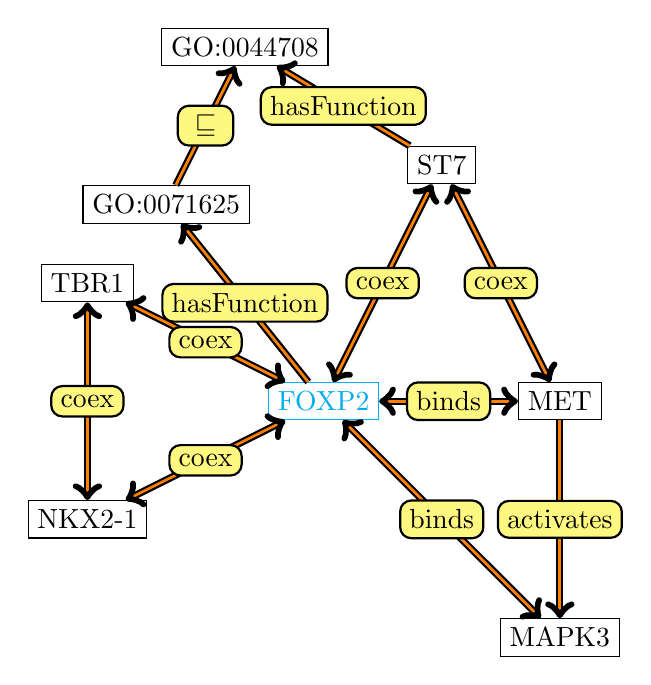
\begin{tikzpicture}
%          \SetUpEdge[lw = 1pt, color = black]
          \GraphInit[vstyle=Shade]
          \tikzset{
            LabelStyle/.style = { rectangle, rounded corners, draw,
              minimum width = 2em, fill = yellow!50,
              text = black },
            VertexStyle/.append style = { inner sep=5pt,
              font = \Large\bfseries},
            EdgeStyle/.append style = {->} }
          
          \SetGraphUnit{5}
          % \tikzset{VertexStyle/.append style={fill}}
          % \tikzset{EdgeStyle/.style={->}}
          \node[draw, color=cyan] (FOXP2) at (0,0) {FOXP2};
          \node[draw] (MET) at (3,0) {MET};
          \node[draw] (ST7) at (1.5,3) {ST7};
          \node[draw] (MAPK3) at (3,-3) {MAPK3};
          \node[draw] (GO0071625) at (-2,2.5) {GO:0071625};
          \node[draw] (GO0044708) at (-1,4.5) {GO:0044708};
          \node[draw] (TBR1) at (-3,1.5) {TBR1};
          \node[draw] (NKX2-1) at (-3,-1.5) {NKX2-1};
          \begin{scope}[/tikz/handle active characters in nodes=false]
          \Edge[label=activates](MET)(MAPK3)
          \Edge[label=hasFunction](FOXP2)(GO0071625)
          \Edge[label=hasFunction](ST7)(GO0044708)
          \Edge[label=$\sqsubseteq$](GO0071625)(GO0044708)

          \tikzset{EdgeStyle/.append style={<->}}
          \Edge[label=binds](FOXP2)(MET)
          \Edge[label=binds](FOXP2)(MAPK3)
          \Edge[label=coex](FOXP2)(TBR1)
          \Edge[label=coex](FOXP2)(NKX2-1)
          \Edge[label=coex](FOXP2)(ST7)
          \Edge[label=coex](MET)(ST7)
          \Edge[label=coex](NKX2-1)(TBR1)
          \end{scope}
          % \tikzset{EdgeStyle/.style={->}}
          % \Edge[label=hf](FOXP2)(GO0044708)
          % \draw[label=binds] (FOXP2) to (MET);
          % \Edge[label=binds](FOXP2)(MET)
          % \Edge[label=activates](MET)(MAPK3)
          % \Edge[label=coexpressed-with](FOXP2)(FOXP4)
          
        \end{tikzpicture}
      }
    \end{column}
    \begin{column}{.4\textwidth}
      \begin{itemize}
      \item FOXP2 is characterized by {\em adjacent} and close nodes
        and edges
      \item different edges may ``transmit'' information differently
      \end{itemize}
    \end{column}
  \end{columns}
      
\end{frame}

\begin{frame}
  \frametitle{Random walks}
%  \frametitle{Neuro-symbolic feature learning}
  \begin{columns}
    \begin{column}{.6\textwidth}
      \resizebox{1\textwidth}{!}{%
        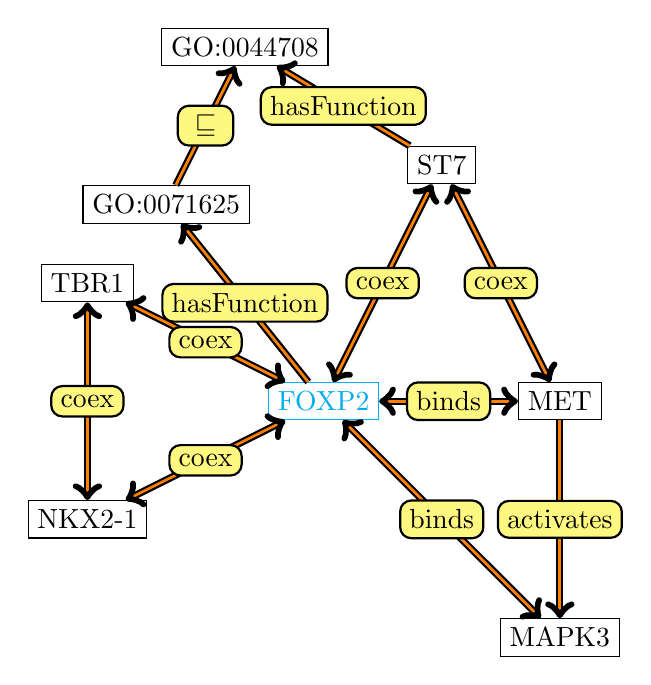
\begin{tikzpicture}
%          \SetUpEdge[lw = 1pt, color = black]
          \GraphInit[vstyle=Shade]
          \tikzset{
            LabelStyle/.style = { rectangle, rounded corners, draw,
              minimum width = 2em, fill = yellow!50,
              text = black },
            VertexStyle/.append style = { inner sep=5pt,
              font = \Large\bfseries},
            EdgeStyle/.append style = {->} }
          
          \SetGraphUnit{5}
          % \tikzset{VertexStyle/.append style={fill}}
          % \tikzset{EdgeStyle/.style={->}}
          \node[draw, color=cyan] (FOXP2) at (0,0) {FOXP2};
          \node[draw] (MET) at (3,0) {MET};
          \node[draw] (ST7) at (1.5,3) {ST7};
          \node[draw] (MAPK3) at (3,-3) {MAPK3};
          \node[draw] (GO0071625) at (-2,2.5) {GO:0071625};
          \node[draw] (GO0044708) at (-1,4.5) {GO:0044708};
          \node[draw] (TBR1) at (-3,1.5) {TBR1};
          \node[draw] (NKX2-1) at (-3,-1.5) {NKX2-1};
          \begin{scope}[/tikz/handle active characters in nodes=false]
          \Edge[label=activates](MET)(MAPK3)
          \Edge[label=hasFunction](FOXP2)(GO0071625)
          \Edge[label=hasFunction](ST7)(GO0044708)
          \Edge[label=$\sqsubseteq$](GO0071625)(GO0044708)

          \tikzset{EdgeStyle/.append style={<->}}
          \Edge[label=binds](FOXP2)(MET)
          \Edge[label=binds](FOXP2)(MAPK3)
          \Edge[label=coex](FOXP2)(TBR1)
          \Edge[label=coex](FOXP2)(NKX2-1)
          \Edge[label=coex](FOXP2)(ST7)
          \Edge[label=coex](MET)(ST7)
          \Edge[label=coex](NKX2-1)(TBR1)
          \end{scope}
          % \tikzset{EdgeStyle/.style={->}}
          % \Edge[label=hf](FOXP2)(GO0044708)
          % \draw[label=binds] (FOXP2) to (MET);
          % \Edge[label=binds](FOXP2)(MET)
          % \Edge[label=activates](MET)(MAPK3)
          % \Edge[label=coexpressed-with](FOXP2)(FOXP4)
          
        \end{tikzpicture}
      }
    \end{column}
    \begin{column}{.4\textwidth}
      \begin{itemize}
      \item precompute the deductive closure:
      \item for all $\phi$: if $\mathcal{KG} \models \phi$, add $\phi$
        to $\mathcal{KG}$
      \end{itemize}
    \end{column}
  \end{columns}
      
\end{frame}

\begin{frame}
  \frametitle{Random walks}
%  \frametitle{Neuro-symbolic feature learning}
  \begin{columns}
    \begin{column}{.6\textwidth}
      \resizebox{1\textwidth}{!}{%
        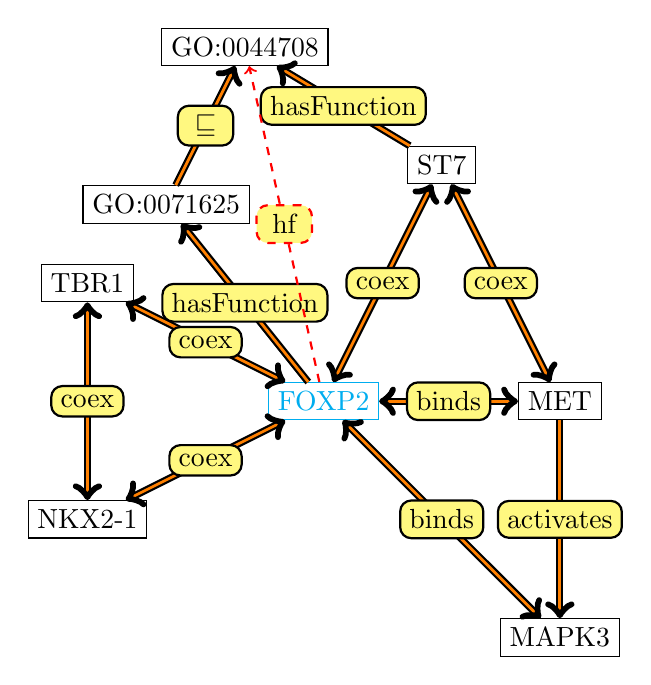
\begin{tikzpicture}
%          \SetUpEdge[lw = 1pt, color = black]
          \GraphInit[vstyle=Shade]
          \tikzset{
            LabelStyle/.style = { rectangle, rounded corners, draw,
              minimum width = 2em, fill = yellow!50,
              text = black },
            VertexStyle/.append style = { inner sep=5pt,
              font = \Large\bfseries},
            EdgeStyle/.append style = {->} }
          
          \SetGraphUnit{5}
          % \tikzset{VertexStyle/.append style={fill}}
          % \tikzset{EdgeStyle/.style={->}}
          \node[draw, color=cyan] (FOXP2) at (0,0) {FOXP2};
          \node[draw] (MET) at (3,0) {MET};
          \node[draw] (ST7) at (1.5,3) {ST7};
          \node[draw] (MAPK3) at (3,-3) {MAPK3};
          \node[draw] (GO0071625) at (-2,2.5) {GO:0071625};
          \node[draw] (GO0044708) at (-1,4.5) {GO:0044708};
          \node[draw] (TBR1) at (-3,1.5) {TBR1};
          \node[draw] (NKX2-1) at (-3,-1.5) {NKX2-1};
          \begin{scope}[/tikz/handle active characters in nodes=false]
          \Edge[label=activates](MET)(MAPK3)
          \Edge[label=hasFunction](FOXP2)(GO0071625)
          \Edge[label=hasFunction](ST7)(GO0044708)
          \Edge[label=$\sqsubseteq$](GO0071625)(GO0044708)

          \tikzset{EdgeStyle/.append style={<->}}
          \Edge[label=binds](FOXP2)(MET)
          \Edge[label=binds](FOXP2)(MAPK3)
          \Edge[label=coex](FOXP2)(TBR1)
          \Edge[label=coex](FOXP2)(NKX2-1)
          \Edge[label=coex](FOXP2)(ST7)
          \Edge[label=coex](MET)(ST7)
          \Edge[label=coex](NKX2-1)(TBR1)

          \tikzset{EdgeStyle/.style={->}}
          \Edge[label=hf, color=red, style=dashed](FOXP2)(GO0044708)
          \end{scope}
          % \tikzset{EdgeStyle/.style={->}}
          % \Edge[label=hf](FOXP2)(GO0044708)
          % \draw[label=binds] (FOXP2) to (MET);
          % \Edge[label=binds](FOXP2)(MET)
          % \Edge[label=activates](MET)(MAPK3)
          % \Edge[label=coexpressed-with](FOXP2)(FOXP4)
          
        \end{tikzpicture}
      }
    \end{column}
    \begin{column}{.4\textwidth}
      \begin{itemize}
      \item precompute the deductive closure:
      \item for all $\phi$: if $\mathcal{KG} \models \phi$, add $\phi$
        to $\mathcal{KG}$
      \end{itemize}
    \end{column}
  \end{columns}
      
\end{frame}


\begin{frame}
  \frametitle{Random walks}
%  \frametitle{Neuro-symbolic feature learning}
  \begin{columns}
    \begin{column}{.6\textwidth}
      \resizebox{1\textwidth}{!}{%
        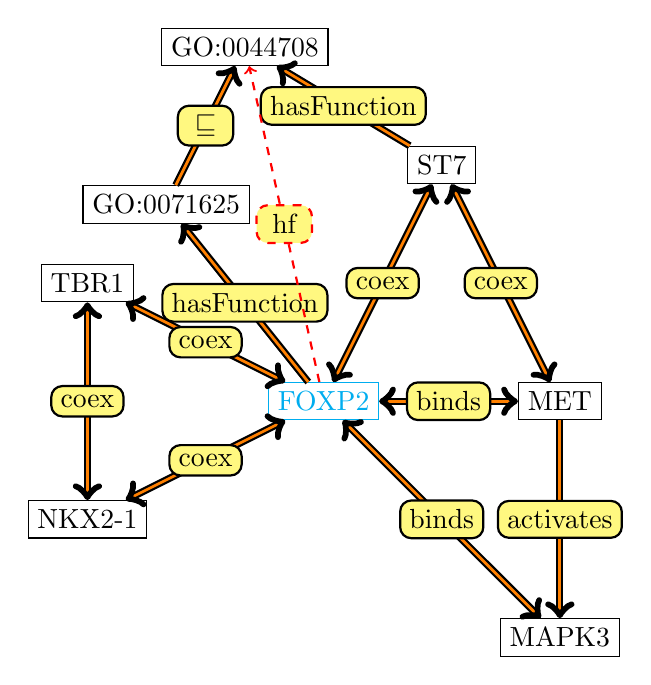
\begin{tikzpicture}
%          \SetUpEdge[lw = 1pt, color = black]
          \GraphInit[vstyle=Shade]
          \tikzset{
            LabelStyle/.style = { rectangle, rounded corners, draw,
              minimum width = 2em, fill = yellow!50,
              text = black },
            VertexStyle/.append style = { inner sep=5pt,
              font = \Large\bfseries},
            EdgeStyle/.append style = {->} }
          
          \SetGraphUnit{5}
          % \tikzset{VertexStyle/.append style={fill}}
          % \tikzset{EdgeStyle/.style={->}}
          \node[draw, color=cyan] (FOXP2) at (0,0) {FOXP2};
          \node[draw] (MET) at (3,0) {MET};
          \node[draw] (ST7) at (1.5,3) {ST7};
          \node[draw] (MAPK3) at (3,-3) {MAPK3};
          \node[draw] (GO0071625) at (-2,2.5) {GO:0071625};
          \node[draw] (GO0044708) at (-1,4.5) {GO:0044708};
          \node[draw] (TBR1) at (-3,1.5) {TBR1};
          \node[draw] (NKX2-1) at (-3,-1.5) {NKX2-1};
          \begin{scope}[/tikz/handle active characters in nodes=false]
          \Edge[label=activates](MET)(MAPK3)
          \Edge[label=hasFunction](FOXP2)(GO0071625)
          \Edge[label=hasFunction](ST7)(GO0044708)
          \Edge[label=$\sqsubseteq$](GO0071625)(GO0044708)

          \tikzset{EdgeStyle/.append style={<->}}
          \Edge[label=binds](FOXP2)(MET)
          \Edge[label=binds](FOXP2)(MAPK3)
          \Edge[label=coex](FOXP2)(TBR1)
          \Edge[label=coex](FOXP2)(NKX2-1)
          \Edge[label=coex](FOXP2)(ST7)
          \Edge[label=coex](MET)(ST7)
          \Edge[label=coex](NKX2-1)(TBR1)

          \tikzset{EdgeStyle/.style={->}}
          \Edge[label=hf, color=red, style=dashed](FOXP2)(GO0044708)
          \end{scope}
          % \draw[label=binds] (FOXP2) to (MET);
          % \Edge[label=binds](FOXP2)(MET)
          % \Edge[label=activates](MET)(MAPK3)
          % \Edge[label=coexpressed-with](FOXP2)(FOXP4)
          
        \end{tikzpicture}
      }
    \end{column}
    \begin{column}{.4\textwidth}
      \begin{itemize}
      \item Exploring the graph:
        \pause
      \item :FOXP2 :binds :MET :coex :ST7 :hasFunction GO:0044708
        \pause
      \item :FOXP2 :hasFunction GO:0071625 subClassOf GO:0044708
        \pause
      \item :FOXP2 :coex :TBR1 :coex :NKX2-1 :coex :TBR1 :coex ...
      \end{itemize}
    \end{column}
  \end{columns}
\end{frame}

\begin{frame}
  \frametitle{Word2Vec}
  Maximize:
  \begin{equation}
    \frac{1}{N} \sum_{n=1}^{N} \sum_{-c\leq j \leq c, j\not=
      0} \log p(w_{n+j}|w_n)
  \end{equation}
  with
  \begin{equation}
    p(w_o | w_i) = \frac{\exp({v'_{w_o}}^T v_{w_i})}{\sum_{w=1}^{W}
      \exp({v'_{w}}^T v_{w_i})}
  \end{equation}
  (at least conceptually; different strategies are used to approximate Eqn. 2)
\end{frame}

\begin{frame}
  \frametitle{Word2Vec and Random Walks}
  \begin{itemize}
  \item random walks ``flatten'' a graph
    \begin{itemize}
    \item walks capture node neighborhood
    \item and generate a ``corpus''
    \end{itemize}
  \item random walks capture graph ``structure''
    \begin{itemize}
    \item hub-nodes, communities, etc.
    \item determine ``importance'' of nodes
    \end{itemize}
  \item embeddings capture co-occurrence
    \begin{itemize}
    \item similar graph neighborhood $\Rightarrow$ similar
      co-occurrence $\Rightarrow$ similar vector
    \end{itemize}
  \item embeddings generate ``feature'' vectors
    \begin{itemize}
    \item functions from symbols (words, labels) into $\Re^n$
    \end{itemize}
  \end{itemize}
\end{frame}

\begin{frame}
  \frametitle{What to do with embeddings?}
  \begin{itemize}
  \item useful for edge prediction, similarity, clustering, as feature
    vectors
    \begin{itemize}
    \item supervised: edge prediction (e.g., SVM, ANN)
      \begin{itemize}
      \item e.g.: find a function $f:\Re^n \times \Re^n \mapsto [0,1]$
        s.t. $\sqrt \frac{\sum_{t=1}^T (\hat{y_t} - y_t)^2}{T}$ (RMSE)
        is minimized for a set of true labels $y_k$
      \end{itemize}
    \item unsupervised: clustering, similarity, visualization
      \begin{itemize}
      \item cosine similarity (for L2-normalized features)
      \item Word2Vec embeddings capture similarity between co-occurrence vectors
      \end{itemize}
    \end{itemize}
  \end{itemize}
\end{frame}

\begin{frame}
  \frametitle{Visualizing embeddings}
%  \frametitle{Neuro-symbolic feature learning}
  \centerline{\includegraphics[width=\textwidth]{graph-tsne.png}}
\end{frame}

\begin{frame}
  \frametitle{Supervised learning}
  \begin{itemize}
  \item feature vectors represent graph neighborhood of nodes
    \begin{itemize}
    \item adjacent nodes and edges
    \item ontology classes (asserted \& inferred)
    \end{itemize}
  \item useful in supervised prediction tasks
  \item relation prediction:
    \begin{itemize}
    \item input: two features vectors (from embedding function)
    \item output: $0$ or $1$ (relation or not)
    \item training data: positive and negative cases
      \begin{itemize}
      \item $R(x,y)$ and $\neg R(x,y)$
      \end{itemize}
    \end{itemize}
  \end{itemize}
\end{frame}

\begin{frame}
  \frametitle{Features: supervised learning}
  \resizebox{\textwidth}{!}{
  \begin{tabular}{@{}lllcccc@{}}\toprule 
      \multirow{2}{*}{Object property} 
      & Source type & Target type &\multicolumn{2}{c}{Without reasoning}&\multicolumn{2}{c}{With reasoning}\\
      &&& F-measure & AUC & F-measure & AUC \\
      \midrule
      has target & Drug & Gene/Protein & 0.94 & 0.97 & 0.94 & 0.98 \\
      has disease annotation & Gene/Protein & Disease & 0.89 & 0.95 & 0.89 & 0.95 \\
      has side-effect$^*$ & Drug & Phenotype & 0.86 & 0.93 & 0.87 & 0.94 \\
      has interaction & Gene/Protein & Gene/Protein & 0.82 & 0.88 & 0.82 & 0.88\\
      has function$^*$ & Gene/Protein & Function & 0.85 & 0.95 & 0.83 & 0.91 \\
      has gene phenotype$^*$  & Gene/Protein & Phenotype & 0.84 & 0.91 & 0.82 & 0.90  \\
      has indication & Drug & Disease & 0.72 & 0.79 & 0.76 & 0.83 \\
      has disease phenotype$^*$  & Disease & Phenotype & 0.72 & 0.78 & 0.70 & 0.77 \\
    \end{tabular}}
\end{frame}

\begin{frame}
  \frametitle{Some limitations}
  \begin{itemize}
  \item ``word''-based (Word2Vec):
    \begin{itemize}
    \item semantics is reduced to co-occurrence in the random
      ``walks''
    \item ``disjointWith'' vs. ``part-of'' vs. ``subClassOf''
    \end{itemize}
  \end{itemize}
\end{frame}

\begin{frame}
  \frametitle{Translating embeddings}
  \centerline{\includegraphics[width=.7\textwidth]{transe-figure.png}}
\end{frame}

\begin{frame}
  \frametitle{Translating embeddings}
  \begin{columns}
    \begin{column}{.6\textwidth}
      \resizebox{1\textwidth}{!}{%
        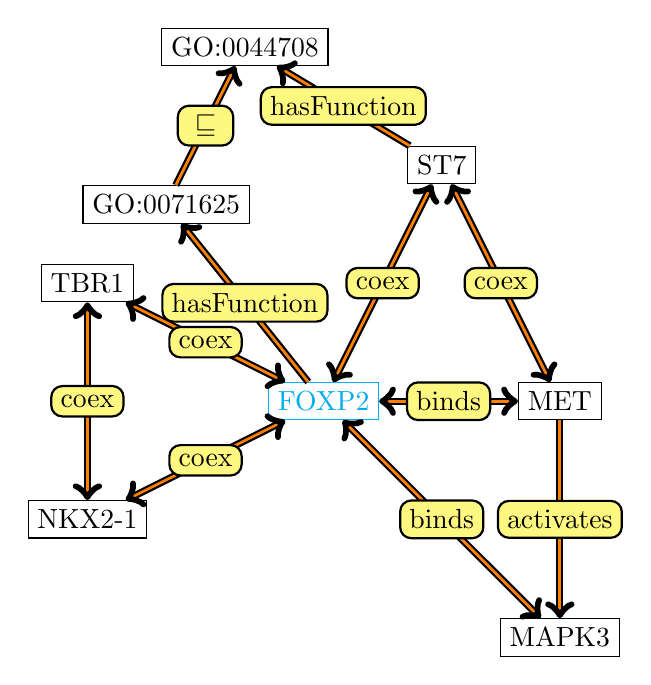
\begin{tikzpicture}
%          \SetUpEdge[lw = 1pt, color = black]
          \GraphInit[vstyle=Shade]
          \tikzset{
            LabelStyle/.style = { rectangle, rounded corners, draw,
              minimum width = 2em, fill = yellow!50,
              text = black },
            VertexStyle/.append style = { inner sep=5pt,
              font = \Large\bfseries},
            EdgeStyle/.append style = {->} }
          
          \SetGraphUnit{5}
          % \tikzset{VertexStyle/.append style={fill}}
          % \tikzset{EdgeStyle/.style={->}}
          \node[draw, color=cyan] (FOXP2) at (0,0) {FOXP2};
          \node[draw] (MET) at (3,0) {MET};
          \node[draw] (ST7) at (1.5,3) {ST7};
          \node[draw] (MAPK3) at (3,-3) {MAPK3};
          \node[draw] (GO0071625) at (-2,2.5) {GO:0071625};
          \node[draw] (GO0044708) at (-1,4.5) {GO:0044708};
          \node[draw] (TBR1) at (-3,1.5) {TBR1};
          \node[draw] (NKX2-1) at (-3,-1.5) {NKX2-1};
          \begin{scope}[/tikz/handle active characters in nodes=false]
          \Edge[label=activates](MET)(MAPK3)
          \Edge[label=hasFunction](FOXP2)(GO0071625)
          \Edge[label=hasFunction](ST7)(GO0044708)
          \Edge[label=$\sqsubseteq$](GO0071625)(GO0044708)

          \tikzset{EdgeStyle/.append style={<->}}
          \Edge[label=binds](FOXP2)(MET)
          \Edge[label=binds](FOXP2)(MAPK3)
          \Edge[label=coex](FOXP2)(TBR1)
          \Edge[label=coex](FOXP2)(NKX2-1)
          \Edge[label=coex](FOXP2)(ST7)
          \Edge[label=coex](MET)(ST7)
          \Edge[label=coex](NKX2-1)(TBR1)
          \end{scope}
          % \tikzset{EdgeStyle/.style={->}}
          % \Edge[label=hf](FOXP2)(GO0044708)
          % \draw[label=binds] (FOXP2) to (MET);
          % \Edge[label=binds](FOXP2)(MET)
          % \Edge[label=activates](MET)(MAPK3)
          % \Edge[label=coexpressed-with](FOXP2)(FOXP4)
          
        \end{tikzpicture}
      }
    \end{column}
    \begin{column}{.4\textwidth}
      \begin{itemize}
        \pause
      \item FOXP2 + binds = MET
        \pause
      \item MAP + activates = MAPK3
        \pause
      \item MET + binds = FOXP2
        \pause
      \item ST7 + hasFunction = {\tt GO:0044708}
        \pause
      \item ...
      \end{itemize}
    \end{column}
  \end{columns}
\end{frame}

\begin{frame}
  \frametitle{Translating embeddings}
  \begin{columns}
    \begin{column}{.6\textwidth}
      \resizebox{1\textwidth}{!}{%
        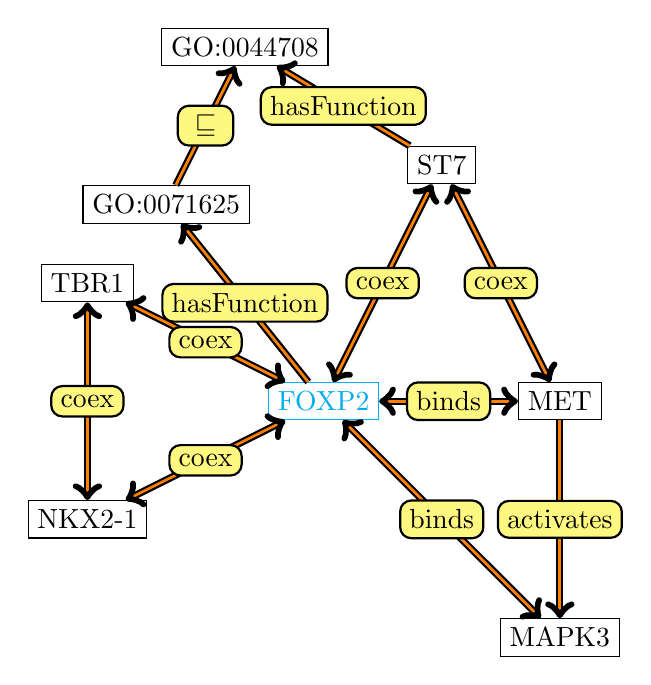
\begin{tikzpicture}
%          \SetUpEdge[lw = 1pt, color = black]
          \GraphInit[vstyle=Shade]
          \tikzset{
            LabelStyle/.style = { rectangle, rounded corners, draw,
              minimum width = 2em, fill = yellow!50,
              text = black },
            VertexStyle/.append style = { inner sep=5pt,
              font = \Large\bfseries},
            EdgeStyle/.append style = {->} }
          
          \SetGraphUnit{5}
          % \tikzset{VertexStyle/.append style={fill}}
          % \tikzset{EdgeStyle/.style={->}}
          \node[draw, color=cyan] (FOXP2) at (0,0) {FOXP2};
          \node[draw] (MET) at (3,0) {MET};
          \node[draw] (ST7) at (1.5,3) {ST7};
          \node[draw] (MAPK3) at (3,-3) {MAPK3};
          \node[draw] (GO0071625) at (-2,2.5) {GO:0071625};
          \node[draw] (GO0044708) at (-1,4.5) {GO:0044708};
          \node[draw] (TBR1) at (-3,1.5) {TBR1};
          \node[draw] (NKX2-1) at (-3,-1.5) {NKX2-1};
          \begin{scope}[/tikz/handle active characters in nodes=false]
          \Edge[label=activates](MET)(MAPK3)
          \Edge[label=hasFunction](FOXP2)(GO0071625)
          \Edge[label=hasFunction](ST7)(GO0044708)
          \Edge[label=$\sqsubseteq$](GO0071625)(GO0044708)

          \tikzset{EdgeStyle/.append style={<->}}
          \Edge[label=binds](FOXP2)(MET)
          \Edge[label=binds](FOXP2)(MAPK3)
          \Edge[label=coex](FOXP2)(TBR1)
          \Edge[label=coex](FOXP2)(NKX2-1)
          \Edge[label=coex](FOXP2)(ST7)
          \Edge[label=coex](MET)(ST7)
          \Edge[label=coex](NKX2-1)(TBR1)
          \end{scope}
          % \tikzset{EdgeStyle/.style={->}}
          % \Edge[label=hf](FOXP2)(GO0044708)
          % \draw[label=binds] (FOXP2) to (MET);
          % \Edge[label=binds](FOXP2)(MET)
          % \Edge[label=activates](MET)(MAPK3)
          % \Edge[label=coexpressed-with](FOXP2)(FOXP4)
          
        \end{tikzpicture}
      }
    \end{column}
    \begin{column}{.4\textwidth}
      \begin{itemize}
      \item FOXP2 + binds - MET = 0
      \item MAP + activates - MAPK3 = 0
      \item MET + binds - FOXP2 = 0
      \item ST7 + hasFunction - {\tt GO:0044708} = 0
      \item ...
      \end{itemize}
    \end{column}
  \end{columns}
\end{frame}

\begin{frame}
  \frametitle{Translating embeddings}
  \centerline{\includegraphics[width=1\textwidth]{transe-algorithm.png}}

  {\tiny Bordes et al. (2013). Translating Embeddings for
    ModelingMulti-relational Data.}
\end{frame}

\begin{frame}
  \frametitle{Some properties of TransE}
  \begin{itemize}
  \item graph-based
    \begin{itemize}
    \item works well on RDF graphs
    \item and ontology graphs
    \end{itemize}
  \item 1:1 relations only
    \begin{itemize}
    \item not suitable for hierarchies (1-N relations)
    \item not suitable for N-N relations
    \item no transitive, symmetric, reflexive relations
    \end{itemize}
  \end{itemize}
\end{frame}

\begin{frame}
  \frametitle{Translating embeddings}
  \centerline{\includegraphics[width=.7\textwidth]{transh-figure.png}}
\end{frame}

\begin{frame}
  \frametitle{Translating embeddings}
  \centerline{\includegraphics[width=.7\textwidth]{transr-figure.png}}
\end{frame}

\begin{frame}
  \frametitle{Translating embeddings}
  \centerline{\includegraphics[width=\textwidth]{loss-functions-kg.png}}
  {\tiny Wang et al. Knowledge Graph Embedding: A Survey ofApproaches and Applications.}
\end{frame}

\begin{frame}
  \frametitle{Beyond graphs}
  \begin{itemize}
  \item so far, all the methods were based on graphs
    \begin{itemize}
    \item ontologies are not graphs!
    \item converting ontologies to graphs loses information
    \item no axioms, no definitions
    \end{itemize}
  \item maybe we won't need the graph?
  \end{itemize}
\end{frame}

\begin{frame}
  \frametitle{Onto2Vec}
  \centerline{\includegraphics[width=\textwidth]{onto2vecflow.png}}
\end{frame}

\begin{frame}
  \frametitle{Combination with text}
  \begin{itemize}
  \item ontologies contain more than axioms:
    \begin{itemize}
    \item labels, synonyms, definitions, authors, etc.
    \end{itemize}
  \item Description Logic axioms != natural language
  \item transfer learning: learn on one domain/task, apply to another
    \begin{itemize}
    \item e.g.: learn on literature, apply to ontologies
    \item words have ``meaning'' in literature, Description Logic
      symbols have ``meaning'' in ontology axioms
    \end{itemize}
  \item Ontologies Plus Annotations 2 Vec (OPA2Vec) combines both
  \end{itemize}
\end{frame}

\begin{frame}
  \frametitle{Ontologies Plus Annotations 2 Vec}
  \centerline{\includegraphics[width=1\textwidth]{opaworkflow16.png}}
\end{frame}

\begin{frame}
  \frametitle{Axioms contribute to prediction tasks: GO and GO-PLUS}
    % \processtable
    % \caption{AUC values of ROC curves for PPI prediction for
    %   GO-Plus and GO using Onto2Vec (cosine similiarity) and
    %   Onto2Vec-NN (neural network).\label{Tab:GOplus}}
    { \begin{tabularx}{\columnwidth}{XXXXXXX}\toprule & {}& {} &
                                                                 Human & Yeast & Arabidopsis\\\midrule
        $GO\_Onto2Vec$ & {} &{}& 0.7660 & 0.7701 & 0.7559 \\
        $GO\_Onto2Vec\_NN$ & {} & {}& 0.8779& 0.8711 & 0.8364 \\
        $GO\_plus\_Onto2Vec$ & {} & {}& 0.7880& 0.7943 & 0.7889 \\
        $GO\_plus\_Onto2Vec\_NN$ &{} & {}& \textbf{0.9021}&\textbf{0.8937} & \textbf{0.8834}\\
        \hline
      \end{tabularx}}{}
\end{frame}

\begin{frame}
  \frametitle{How to overcome the semantic gap?}
  \begin{itemize}
  \item none of the models discussed above are truly ``semantic''
    \begin{itemize}
    \item all syntactic
    \item graph-based or based on axioms
    \end{itemize}
    \pause
  \item what do we actually mean by ``semantics''?
    \begin{itemize}
    \pause
    \item formal definition of ``truth'' relies on ``models''
    \pause
    \item universal algebra over formal languages (with signature
      $\Sigma$)
    \end{itemize}
  \end{itemize}
\end{frame}

\begin{frame}
  \frametitle{Description Logic EL++}
  \centering
  \resizebox{.8\textwidth}{!}{
    
    \begin{tabular}{|p{1.7cm}|c|p{3.7cm}|}
      \hline
      {\bf} Name & Syntax & Semantics \\
      \hline
      top & $\top$ & $\Delta^{\mathcal{I}}$ \\
    \hline
    bottom & $\bot$ & $\emptyset$ \\
    \hline
    nominal & $\{ a \} $ & $\{ a^{\mathcal{I}} \}$ \\
    \hline
    conjunction & $C \sqcap D$ & $ C^{\mathcal{I}} \cap
                                 D^{\mathcal{I}}$ \\
    \hline
    existential restriction & $\exists r.C$ & $ \{ x \in
                                              \Delta^{\mathcal{I}} |
                                              \exists y \in
                                              \Delta^{\mathcal{I}} :
                                              (x,y) \in
                                              r^{\mathcal{I}} \land y
                                              \in C^{\mathcal{I}} \} $
    \\
    \hline
    generalized concept inclusion & $C \sqsubseteq D$ &
                                                        $C^{\mathcal{I}}
                                                        \subseteq
                                                        D^{\mathcal{I}}$
    \\
    \hline
    role inclusion & $r_1 \circ ... \circ r_n \sqsubseteq r$ &
                                                               $r_1^{\mathcal{I}}
                                                               \circ
                                                               ... \circ
                                                               r_n^{\mathcal{I}}
                                                               \subseteq
                                                               r^{\mathcal{I}}$
    \\
    \hline
    
  \end{tabular}
}
\end{frame}

\begin{frame}
  \frametitle{Models}
  \begin{itemize}
  \item Interpretations and $\Sigma$-structures
  \item Model $\mathfrak{A}$ of a formula $\phi$: $\phi$ is true in
    $\mathfrak{A}$ ($\mathfrak{A} \models \phi$) 
  \item Theory $T$: set of formulas
  \item $\mathfrak{A}$ is a model of $T$ if $\mathfrak{A}$ is a model
    of all formulas in $T$
  \item Ontologies are (special kinds of) theories
  \end{itemize}
\end{frame}

\begin{frame}
  \frametitle{EL Embeddings}
  \begin{itemize}
  \item given a theory/ontology $T$ with signature $\Sigma(T)$
  \item aim: find $f_e: \Sigma(T) \mapsto \Re^n$ s.t. $f_e(\Sigma(T))$
    is a model of $T$ ($f_e(\Sigma(T)) \models T$)
    \pause
  \item more general: find an algorithm that maps symbols (signatures)
    into $\Re^n$ so that the {\em semantics} of the symbol (expressed
    through axioms and explicit in model structures) is preserved
    \pause
  \item any consistent EL++ theory has infinite models
    \pause
  \item any consistent EL++ theory has models in $\mathbb{R}^n$
    (Loewenheim-Skolem, upwards)
  \end{itemize}
\end{frame}

\begin{frame}
  \frametitle{Key idea}
  \begin{itemize}
  \item for all $r \in \Sigma(T)$ and $C \in \Sigma(T)$, define
    $f_e(r)$ and $f_e(C)$
  \item $f_e(C)$ maps to points in an open $n$-ball such that
    $f_e(C) = C^{\mathcal{I}}$:
    $C^{\mathcal{I}} = \{ x \in \mathbb{R}^n | \norm{f_e(C) - x} <
    r_e(C) \}$
    \begin{itemize}
    \item these are the {\em extension} of a class in $\Re^n$
    \end{itemize}
  \item $f_e(r)$ maps a binary relation $r$ to a vector such that
    % the set of tuples ($\mathbb{R}^n \times \mathbb{R}^n$) with
    % $f_e(r) = r^{\mathcal{I}}$:
    $r^{\mathcal{I}} = \{ (x,y) | x + f_e(r) = y \}$
    \begin{itemize}
    \item that's the TransE property for {\em individuals}
    \end{itemize}
  \item use the axioms in $T$ as constraints
  \end{itemize}
\end{frame}

\begin{frame}
  \frametitle{Algorithm}
  \begin{itemize}
  \item normalize the theory:
    \begin{itemize}
    \item every \el theory can be expressed using four normal forms
      (Baader et al., 2005)
    \end{itemize}
  \item eliminate the ABox: replace each individual symbol with a
    singleton class: $a$ becomes $\{a\}$
  \item rewrite relation assertions $r(a,b)$ and class
    assertions $C(a)$ as $\{ a \} \sqsubseteq \exists r.\{ b \}$ and
    $\{ a \} \sqsubseteq C$
    \begin{itemize}
    \item something to remember for the next class-vs-instance discussion?
    \end{itemize}
  \item normalization rules to generate:
    \begin{itemize}
    \item $C \sqsubseteq D$
    \item $C \sqcap D \sqsubseteq E$
    \item $C \sqsubseteq \exists R.D$
    \item $\exists R.C \sqsubseteq D$
    \end{itemize}
  \end{itemize}
\end{frame}

\begin{frame}
  \frametitle{Algorithm: loss functions}
  \begin{equation}
    \label{eqn:nf1}
    \begin{split}
      & loss_{C \sqsubseteq D}(c,d) = \\
      & \max(0, \norm{f_\eta(c) - f_\eta(d)} + r_\eta(c) - r_\eta(d) - \gamma) \\
      & + |\norm{f_\eta(c)} - 1| + |\norm{f_\eta(d)} - 1|
    \end{split}
  \end{equation}
\end{frame}

\begin{frame}
  \frametitle{Algorithm: loss functions}
  Let
  $h=\frac{r_\eta(c)^2-r_\eta(d)^2+\norm{f_\eta(c) -
      f_\eta(d)}^2}{2\norm{f_\eta(c) - f_\eta(d)}}$, then the center and
  radius of the smallest $n$-ball containing the intersection of
  $\eta(C)$ and $\eta(D)$ are
  $f_\eta(c)+\frac{h}{\norm{f_\eta(c) -
      f_\eta(d)}}(f_\eta(d)-f_\eta(c))$ and $\sqrt{r_\eta(c)^2-h^2}$.
\end{frame}

\begin{frame}
  \frametitle{Algorithm: loss functions}
  \begin{equation}
    \label{eqn:nf3}
    \begin{split}
      & loss_{C \sqsubseteq \exists R.D}(c,d,r) = \\
      & \max(0, \norm{f_\eta(c) + f_\eta(r) - f_\eta(d)}  + r_\eta(c) - r_\eta(d) - \gamma) \\
      & + |\norm{f_\eta(c)} - 1| + |\norm{f_\eta(d)} - 1|
    \end{split}
  \end{equation}
\end{frame}

\begin{frame}
  \frametitle{Algorithm: loss functions}
  \begin{equation}
    \label{eqn:nf4}
    \begin{split}
      & loss_{\exists R.C \sqsubseteq D}(c,d,r) = \\
      & \max(0, \norm{f_\eta(c) - f_\eta(r) - f_\eta(d)} - r_\eta(c) - r_\eta(d) - \gamma) \\
      & + |\norm{f_\eta(c)} - 1| + |\norm{f_\eta(d)} - 1|
    \end{split}
  \end{equation}
\end{frame}

\begin{frame}
  \frametitle{Algorithm: loss functions}
  \begin{equation}
    \label{eqn:disjoint}
    \begin{split} 
      &loss_{C \sqcap D \sqsubseteq \bot}(c,d,e) = \\
      & \max(0, r_\eta(c) + r_\eta(d) - \norm{f_\eta(c) - f_\eta(d)} + \gamma) \\
      & + |\norm{f_\eta(c)} - 1| + |\norm{f_\eta(d)} - 1|
    \end{split}
  \end{equation}
\end{frame}

\begin{frame}
  \frametitle{Algorithm: loss functions}
  \centerline{\includegraphics[width=1\textwidth]{ellosses.pdf}}
\end{frame}

\begin{frame}
  \frametitle{EL Embeddings}
  \begin{eqnarray}
    & Male & \sqsubseteq Person \\
    & Female & \sqsubseteq Person \\
    & Father & \sqsubseteq Male \\
    & Mother & \sqsubseteq Female \\
    & Father & \sqsubseteq Parent \\
    & Mother & \sqsubseteq Parent \\
    & Female \sqcap Male & \sqsubseteq \bot \\
    & Female \sqcap Parent & \sqsubseteq Mother \\
    & Male \sqcap Parent & \sqsubseteq Father \\
    & \exists hasChild.Person & \sqsubseteq Parent \\
    & Parent & \sqsubseteq Person \\
    & Parent & \sqsubseteq \exists hasChild.\top
               \label{famlast}
               % & Person & \sqsubseteq \top
  \end{eqnarray}
\end{frame}

\begin{frame}
  \frametitle{EL Embeddings}
  \centerline{\animategraphics[loop,controls,width=.7\textwidth]{12}{embeds-frame-}{0}{99}}
  \begin{itemize}
  \item model with $\Delta = R^n$
  \item support quantifiers, negation, conjunction,...
  \end{itemize}
  {\tiny IJCAI 2019}
\end{frame}

\begin{frame}
  \frametitle{Zero-shot prediction with EL Embeddings}
  \begin{itemize}
  \item zero-shot prediction:
    \begin{itemize}
    \item no instance of class $C$ is observed
      \begin{itemize}
      \item e.g., no protein has {\em ever} been observed with function $C$
      \item e.g., no individual has {\em ever} been observed with disease $C$
      \end{itemize}
    \item zero-shot prediction: predict instances of $C$
      \begin{itemize}
      \item assumption: $C$ is used in axioms, e.g., $C \sqsubseteq
        \exists R.D$ or $C \equiv A \sqcap B$
      \end{itemize}
    \end{itemize}
  \item no training data
    \begin{itemize}
    \item can we exploit axioms and entailment within the embedding space?
    \end{itemize}
  \end{itemize}
\end{frame}

\begin{frame}
  \frametitle{Zero-shot prediction with EL Embeddings}

  \centerline{\includegraphics[width=1\textwidth]{deepgozero-eps-converted-to.pdf}}

  \vfill
  {\tiny
    Kulmanov \& Hoehndorf, DeepGOZero: Improving protein function
    prediction from sequence and zero-shot learning based on ontology
    axioms. ISMB, 2022.}
\end{frame}

% \begin{frame}
%   \frametitle{Zero shot protein function prediction}
%   \centerline{
%     \includegraphics[width=.49\textwidth]{annot-terms-eps-converted-to.pdf}
%     \includegraphics[width=.49\textwidth]{zeroshot.pdf}
%     }
  
% \end{frame}

\begin{frame}
  \frametitle{Zero-shot prediction: more general}
  \begin{block}{Embedding}
    An embedding is a map (morphism) from one mathematical structure
    $X$ into another structure $Y$:\\$f : X \xhookrightarrow{} Y$\\
    such that $X$ is preserved in $Y$.
  \end{block}
  \pause
  \begin{itemize}
  \item existence of $f^{-1}$ 
    \begin{itemize}
    \item inverse embedding
    \item allows ``extraction'' of $X$ from $Y$
    \end{itemize}
  \item formulation of the prediction problem in $X$
    \begin{itemize}
    \item e.g., classification: $X \sqsubseteq \exists R.Y$
    \item loss expressed in terms of $f^{-1}$
    \end{itemize}
  \item joint embedding of $X$ and $Z$ in $Y$
    \begin{itemize}
    \item $Z$ is a third structure providing external information
    \end{itemize}
  \end{itemize}
\end{frame}

\begin{frame}
  \frametitle{mOWL}
  \begin{itemize}
  \item high-performance software library for machine learning with
    Semantic Web (OWL) ontologies
  \item ontology embeddings, zero-shot, constrained optimization
  \item contains
    \begin{itemize}
    \item graph generation (DL2Vec, OWL2Vec*, Taxonomy)
    \item graph embedding (random walk + word2vec, node2vec, various
      knowledge graph embedding methods from PyKEEN)
    \item model-based embeddings (ELEm, EMEl, ELBE)
    \item category-theoretical embeddings
    \item FuzzFuzzFuzz ALC embeddings
    \end{itemize}
  \item Algorithms written in Python + Scala (OWLAPI), tuned for performance
  \end{itemize}
  \url{https://github.com/bio-ontology-research-group/mowl}
\end{frame}

\begin{frame}
  \frametitle{Hands-on part}
  There is a notebook available that shows how to use mOWL with all
  the methods introduced here. Run the code in the Notebook. When
  complete, change the task from prediction of PPIs to the prediction
  of gene--disease associations as in the Semantic Similarity
  notebook.
\end{frame}

\end{document}
%%% Local Variables:
%%% mode: latex
%%% TeX-master: t
%%% End:
